Rozdział \ref{subsec:dwuwymiarowe_kopuly_probal} pokazał, że kopuły można intuicyjnie rozumieć jako modele zależności. W tej sekcji spojrzymy na nie z dualnej perspektywy, co pozwoli nam zdefiniować użyteczne narzędzia do analizy charakteru tej zależności.

\begin{df}[Gęstość kopuły]
	Niech $C$ będzie $d$-wymiarową (jednostajnie ciągłą) kopułą. Gęstością tej kopuły nazywamy funkcję
	\begin{equation}
		c(u_1, \dots, u_d) = \frac{\partial^d}{\partial u_1\dots \partial u_d}C(u_1, \dots, u_d).
		\label{eq:copula_density}
	\end{equation}
\end{df}

Widzimy, że równanie \ref{eq:copula_density} jest jedynie przeniesieniem terminu gęstości rozkładu na grunt kopuł. Zanim zaczniemy wizualizować gęstości konkretnych kopuł, warto wspomnieć, że Sklar w \cite{Sklar_Theorem} podaje również alternatywną wersję swojego twierdzenia o istnieniu kopuły, tym razem w języku gęstości. Sens i zastosowania twierdzenia pozostają takie same jak przy \ref{thm:sklar_theorem}.
\begin{thm}[Twierdzenie Sklara: gęstość kopuły]
	Niech $X$ będzie $d$-wymiarowym wektorem losowym o dystrybuancie rozkładu łącznego $F$, oraz rozkładami brzegowymi $F_i$, $i=1, \dots, d$. Wtedy rozkład łączny może być wyrażony jako		$$F(x_1, \dots, x_d) = C(F_1(x_1), \dots, F_d(x_d)),$$
	lub równoważnie w terminach gęstości poprzez:
	$$ f(x_1, \dots, x_d) = c(F_1(x_1), \dots, F_d(x_d))\cdot f_1(x_1)\dots f_d(x_d),$$
	dla pewnej $d$-wymiarowej kopuli $C$, o gęstości $c$. Dla rozkładów bezwzględnie ciągłych, kopuła $C$ jest jednoznacznie określona.\\
	Zachodzi również twierdzenie odwrotne: kopuła związana z wielowymiarowym rozkładem $F$ o rozkładach brzegowych $F_1, \dots F_d$ może być wyrażona jako:
	$$C(u_1, \dots, u_d) = F(F_1^{-1}(u_1), \dots, F_d^{-1}(u_d)),$$
	a jej gęstość wyraża się poprzez:
	$$c(u_1, \dots, u_d) = \frac{f(F_1^{-1}(u_1), \dots, F_d^{-1}(u_d))}{f_1(F_1^{-1}(u_1))\dots f_d(F_d^{-1}(u_d))}$$
	\label{thm:sklar_theorem_density}
\end{thm}

Resztę rozdziału stanowić będzie opis rodzin kopuł o istotnych zastosowaniach w praktyce.\\

\underline{Kopuła produktowa}\\

Gęstość kopuły produktowej otrzymujemy różniczkując jej dystrybuantę:
$$ c(u, v) =\frac{\partial^2}{\partial u\partial v}C(u, v) = 1. $$ 

\begin{figure}[h]
	\centering
	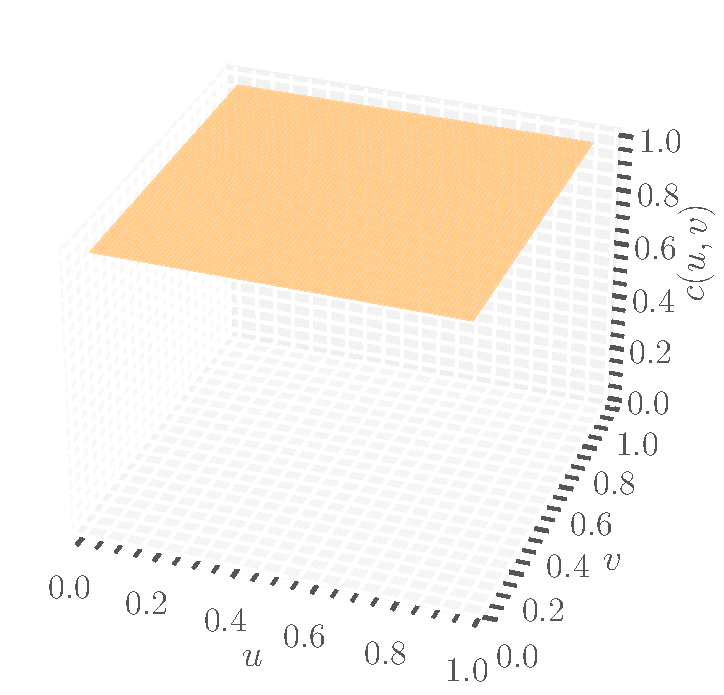
\includegraphics[width=0.4\linewidth]{01_IndependenceCopula_density}
	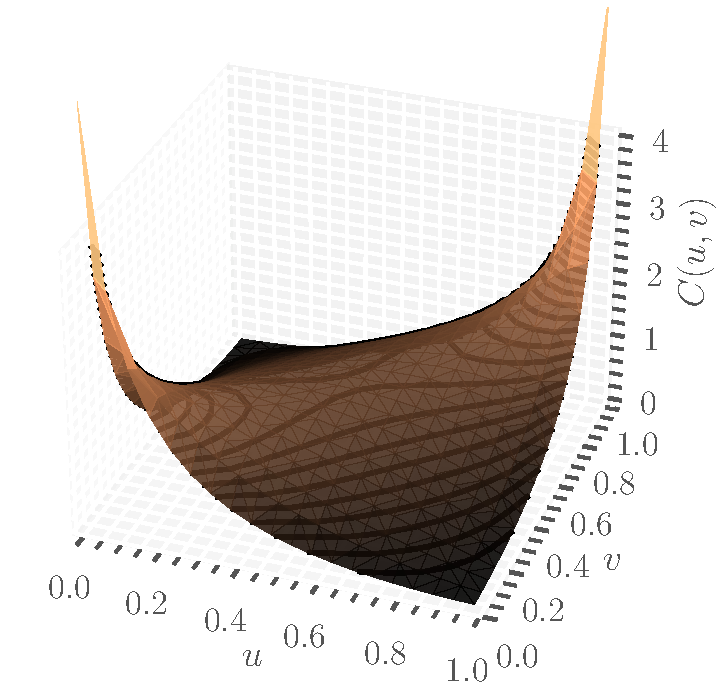
\includegraphics[width=0.4\linewidth]{01_GaussianCopula_density}
	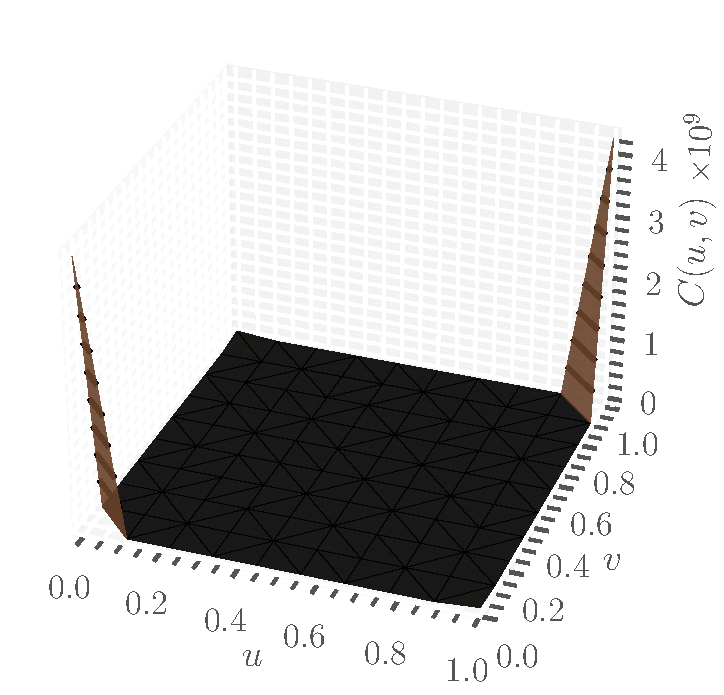
\includegraphics[width=0.4\linewidth]{01_StudentCopula_density}
	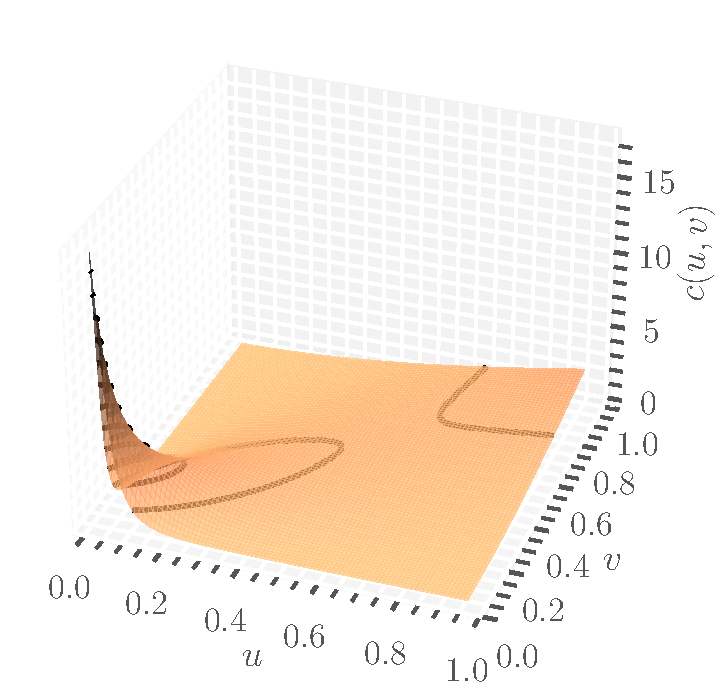
\includegraphics[width=0.4\linewidth]{01_ClaytonCopula_density}
	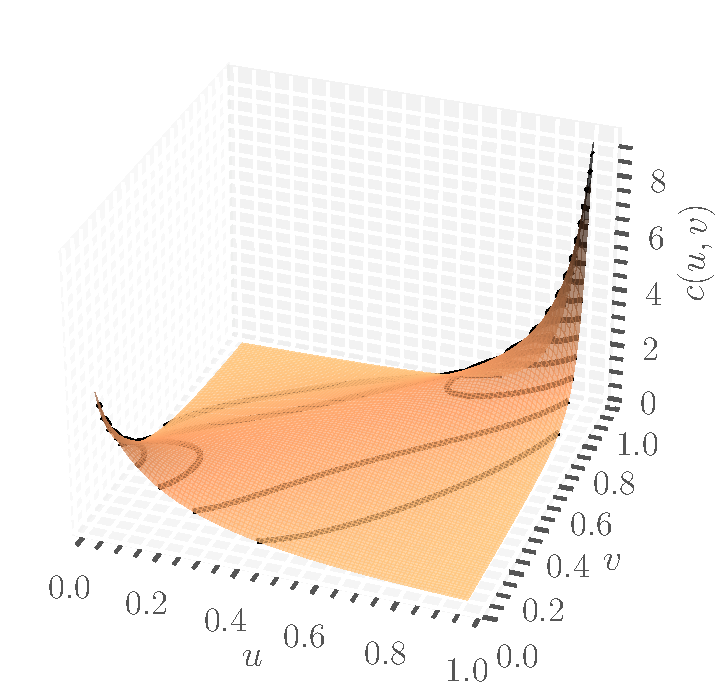
\includegraphics[width=0.4\linewidth]{01_GumbelCopula_density}
	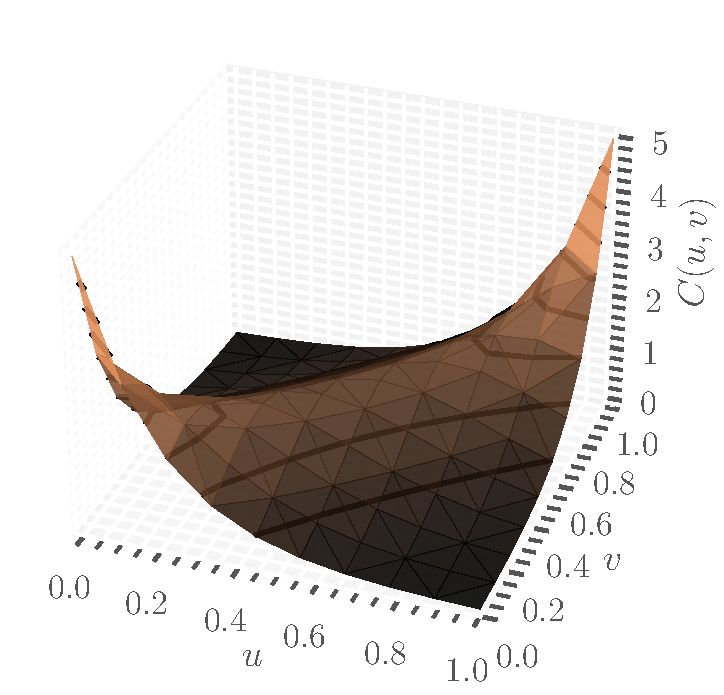
\includegraphics[width=0.4\linewidth]{01_FrankCopula_density}
	
	\caption{Gęstości wybranych kopuł.\label{fig:copula_densities}}
\end{figure}
